
\chapter{Technical choice }
\label{chap:choice}
During this project I made some technical choice. I will explain in this chapter which choice I take and why.

\section{Type of communication}

First of all, I had to find the best way to integrate the simulator in \umld. Because I want to keep the possibility to change the simulator I have decided to put the simulator in a separate thread with a communication by socket. In this way, I had the possibility to change the simulator without changing everything in the plugin, and even start the simulator outside the plugin.

Afterwards, I have to find the best way to realize the communication enter the simulator and the plugin. After list all type of communication enter process with their advantages and their drawback, I decided to chose a socket communication.%, and send message only formatted as json object.

% A lot of type of communication inter process Ire suggested to create a discussion enter the plugin and the simulator. But I will present only the most consistent with their advantages and their drawbacks.

% The communication is the most important part of this project, because that will implement the interface between the two software.


\subsection{Socket}

This next table exhibit advantages and drawback of socket. You can find on appendix \ref{annex:choice} the list of all other type of communication consider. I chose socket instead of other type of communication because it has a better ratio of Advantages/Drawback for this work.
~\\

\begin{tabular}{|p{0.45\textwidth}||p{0.45\textwidth}|}
  \hline
  \textbf{Advantages}&\textbf{Drawback}\\
  \hline
  Work with every language (python, java, ...) & Message need to be formatted\\
  \hline
  Allow communications enter process which don't use the same language& Not very fast\\
  \hline
  Work on all platform (Windows, Linux, OSX)&\\
  \hline
\end{tabular}


\section{Type of message}

Now I have chosen socket to communicate enter the plugin and the simulator, I have to choose which type of object I will send by this socket. In fact, socket message need to be formatted and it exist many way to do that.

In the same way, I list the type of message that I could send, and only three were relevant.

\begin{itemize}
\item String
\item Java object
\item Json message
\end{itemize}

Because String doesn't permit modularity and Java object require to use java for the simulator layer, I chose Json. Moreover, Json are send like String but with a formatted type.

To do that I use a library which permit to manipulate Json object in Java. I found it on Github \cite{json}.
~\\

Our json object are constructed like this:
~\\

plugin \overrightarrow{} simulator
\begin{lstlisting}[style=json]
  JsonPluginToSimulator = {
    initialize : boolean
    play : boolean
    stop : boolean
    restart : boolean
    random : boolean
    reload : boolean
    reloadPath : string
    state : string
  }
\end{lstlisting}

~\\

simulator \overrightarrow{} plugin
\begin{lstlisting}[style=json]
  JsonSimulatorToPlugin = {
    transitions : ["transition1", ...]
    error : boolean
    errorMessage : string
    currentClass : string
    currentStates : [
    {
      class : string
      instance : [
      {
        nom : string
        state : ["state1",...]
      }
      ...
      ]
    }
    ...
    ]
  }

\end{lstlisting}


\section{Overview of the project}

With this choice, it is possible to better understand how the project is construct. The project consist in create a plugin for \umld and a communication layer for the simulator. The plugin communicate to the communication layer with socket and json. The plugin receive the data send from the simulator, analyze them, display them, and send instruction to the simulator.

The figure \ref{fig:project} resume its. By default, the simulator and the communication layer are started by the plugin. So, they are inside \umld but it is possible to put them outside because after the start of their thread they communicate only by socket. In this way, We have a default comportment which is user-friendly because the user don't have to launch an other software, but we can consider that the simulator is outside the plugin. That is why on the figure \ref{fig:project} the simulator is represented outside.

\begin{figure}[h]
  \centering
  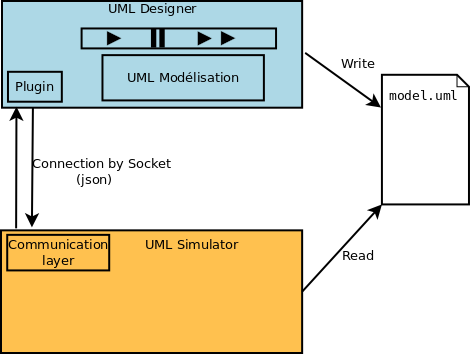
\includegraphics[width=\linewidth]{project}
  \caption{overview of the project}
  \label{fig:project}
\end{figure}



%%% Local Variables:
%%% mode: latex
%%% TeX-master: "../rapport_de_base"
%%% End:
